% !TeX root = ../praktikum.tex
% !TeX encoding = UTF-8
% !Tex spellcheck = de_DE


Anhand der Messdaten aus der Gleichstrommessung, abgebildet in Graphik \ref{fig:full_range_dc} und \ref{fig:2T_range_dc}, wurde die Dichte der Ladungsträger im 2DEG, sowie deren Beweglichkeit bestimmt.

\subsubsection{Näherung über die Hall-Spannung}
\label{ch:naeherung_hall}

Zunächst wurde die Steigung der Hall-Spannung mittels linearer Regression aus dem klassischen Bereich der Messdaten zwischen \unit[-2]{T} und \unit[2]{T} anhand der Formel $ b=\niced{U_{Hall}}{B} $  
bestimmt: \\

$ \d{U_{Hall}}{B} = \frac{m^2}{s} $  %TODO: ZAHLENWERTE! 
\\
Hieraus ließ sich mit der Formel 
\\
$n_s=\frac{I}{e}\frac{1}{\frac{dU_{Hall}}{dB}}$ 
\\
und dem bekannten Strom von $I=\unit[100]{nA}$ die Ladungsträgerdichte des 2DEG berechnen: 
\\
$n_s= \frac{1}{cm^2}$    %TODO: ZAHLENWERTE!
\\
Mit den Bekannten Maßen der Probe wurde anschließend die Beweglichkeit der Ladungsträger bestimmt. Dies erfolgte anhand der Formel \\
$\mu=\frac{1}{n_se}\frac{I}{U_{xx}}\frac{L}{W}$
\\
und mit den Probenmaßen von $600\mu m$ für die Länge L und $100\mu m$  für die Breite B. \\

$\mu= \frac{cm^2}{Vs}$  %TODO: ZAHLENWERTE!

\subsubsection{Näherung über die Shubnikov-de Haas-Oszillation}
\label{ch:naeherung_sdho}

Eine Alternative Möglichkeit, die Ladungsträgerdichte zu berechnen, erfolgt über die Shubnikov-de Haas-Oszillation. Hierzu wurde die Längsspannung über der Probe 
%$U_{Längs}$
 gegen $\frac{1}{B}$ aufgetragen und jedem Minimum der Oszillation ein Füllfaktor $\nu$ zugeordnet. Dies ist in Graphik %TODO: GRAPHIK 
zu sehen. 

Mit der Steigung der Geraden von $b=...$  %TODO: ZAHLENWERTE!
ließ sich analog zur Näherung über die Hallspannung mit Gleichung %TODO: REF! 
die Ladungsträgerdichte bestimmen:
\\
$n_s= \frac{1}{cm^2}$  %TODO: ZAHLENWERTE!
\\
So ergibt sich aus Gleichung %TODO: REF! 
für die Beweglichkeit:
\\
$\mu= \frac{cm^2}{Vs}$  %TODO: ZAHLENWERTE! 


\begin{figure}[h]
	\centering
	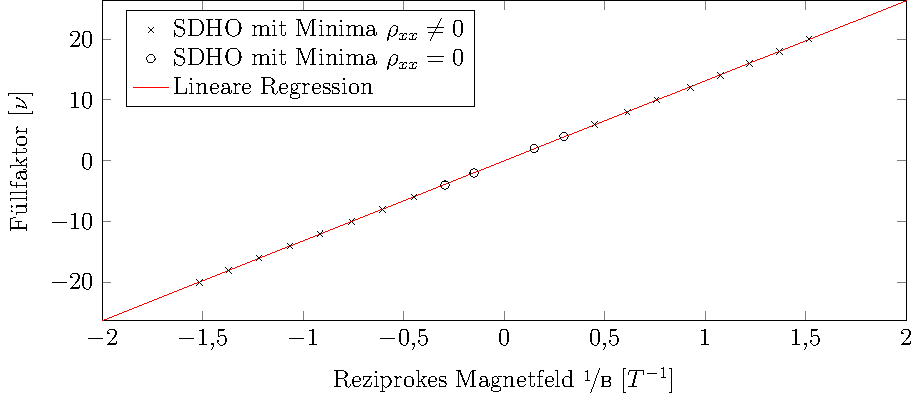
\includegraphics{graphs/dc/auswertung.pdf}
	\caption[Auswertung Füllfaktor Gleichstrommessung]{
		Auswertung Füllfaktor Gleichstrommessung.
	}
	\label{fig:dc_ausw}
\end{figure}

\begin{equation}s
\nu= A\cdot x=(13.1462 \pm 0.0190)T \cdot \nicefrac{1}{B}
\end{equation}